% Diagrama de bloques del lazo cerrado de control de temperatura
\shorthandoff{<>}% babel-spanish activa < y >, que TikZ necesita
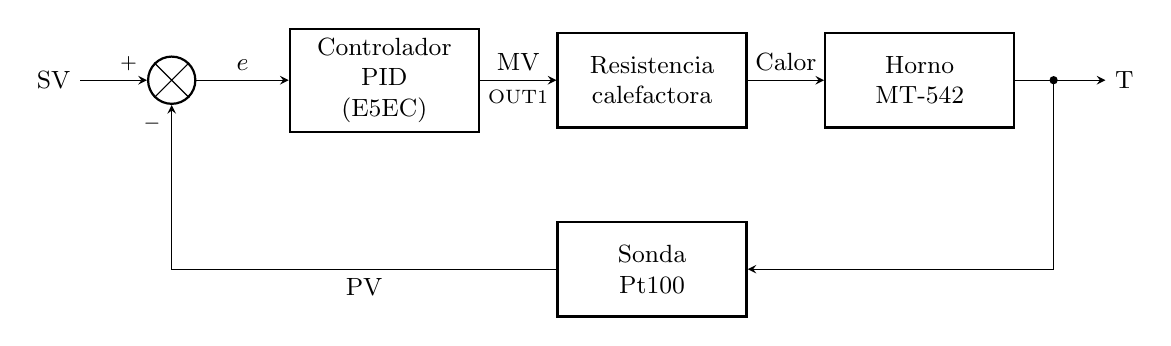
\begin{tikzpicture}[font=\small, >=stealth,
		bloque/.style={draw, thick, minimum height=1.2cm, minimum width=2.4cm, align=center},
		suma/.style={draw, thick, circle, minimum size=0.6cm, inner sep=0pt}]
	\node (sv) at (0,0) {SV};
	\node[suma] (s) at (1.5,0) {};
	\draw (s.north west) -- (s.south east) (s.north east) -- (s.south west);
	\node[bloque] (c) at (4.2,0) {Controlador\\PID\\(E5EC)};
	\node[bloque] (a) at (7.6,0) {Resistencia\\calefactora};
	\node[bloque] (p) at (11,0) {Horno\\MT-542};
	\node (t) at (13.6,0) {T};
	\node[bloque] (m) at (7.6,-2.4) {Sonda\\Pt100};

	\draw[->] (sv) -- (s.west) node[above left, font=\scriptsize]{$+$};
	\draw[->] (s.east) -- node[above]{$e$} (c.west);
	\draw[->] (c.east) -- node[above]{MV} node[below, font=\scriptsize]{OUT1} (a.west);
	\draw[->] (a.east) -- node[above]{Calor} (p.west);
	\draw[->] (p.east) -- (t.west);
	\draw[->] (12.7,0) |- (m.east);
	\draw[->] (m.west) -| node[pos=0.25, below]{PV} (s.south);
	\node[font=\scriptsize] at (1.25,-0.55) {$-$};
	\fill (12.7,0) circle (1.5pt);
\end{tikzpicture}
\shorthandon{<>}
